\documentclass[]{llncs}
\usepackage{graphicx}

%\documentclass{article}
\usepackage{mathtools}
\usepackage{times}  % DO NOT CHANGE THIS
\usepackage{helvet} % DO NOT CHANGE THIS
\usepackage{courier}  % DO NOT CHANGE THIS
\usepackage[hyphens]{url}  % DO NOT CHANGE THIS
\usepackage{arydshln}
\usepackage{mathptmx}
\usepackage{amsmath}
\usepackage{bm}
\usepackage[english]{babel}
\usepackage[utf8]{inputenc}
\usepackage{algorithm}
\usepackage{epstopdf}
\usepackage{booktabs}
\usepackage{multirow}
\usepackage{siunitx}
\usepackage{rotating}
\usepackage{hyperref}
\usepackage[utf8]{inputenc}
\usepackage[T1]{fontenc}
\usepackage{mathtools}
\usepackage[thinc]{esdiff}
%\usepackage[algo2e]{algorithm2e}
%\usepackage{arevmath}     % For math symbols
\usepackage[noend]{algpseudocode}
\urlstyle{rm} % DO NOT CHANGE THIS
\def\UrlFont{\rm}  % DO NOT CHANGE T
% Used for displaying a sample figure. If possible, figure files should
% be included in EPS format.
%
% If you use the hyperref package, please uncomment the following line
% to display URLs in blue roman font according to Springer's eBook style:
% \renewcommand\UrlFont{\color{blue}\rmfamily}

\pagestyle{plain}
\setcounter{page}{1}
\pagenumbering{arabic}

\DeclareMathOperator {\argmax}{argmax} 

\begin{document}

\title{Adaptive Dynamics for the Direct Actions Strategy Approach}

\author{Frances Cameron-Muller, Supervisor: Dr. Julian Garcia}

\institute{Monash University}

\maketitle    

\section{Adaptive Dynamics for Once Off Stag Hunt Game}

Let $x_i \in [0,1]$ be the probability that agent i cooperates. \\
The Stag Hunt Payoff matrix is 
\[
  \begin{pmatrix} 
   R & S  \\
   T & P  
   \end{pmatrix} 
\]
with $ R > T \geq P > S $ \\
\\
Let $ \Pi ( y, x_{-} )$ be the payoff function of playing a strategy y against the rest of the population playing the strategy x. 
\[
\Pi ( y, x_{-} ) = R x y + S (1-x) y +  T x (1-y) + P (1-x) (1-y)
\]
\\
The invasion fitness of a rare mutant strategy y in a population that consists of only strategy x is given by 
\[
f_x(y) = \Pi ( y, x_{-} ) - \Pi ( x, x_{-} )
\]
\begin{multline}
f_x(y) = R x y + S (1-x) y +  T x (1-y) + P (1-x) (1-y) \\ - R x^2 - S (1-x) x - T x (1-x) - P (1-x) (1-x)
\end{multline}
\[
D(x) = \diffp*{f_x(y)}{y}{y=x}
\]
\[
D(x) = (R - S - T +P) x + (S-P)
\]
\\
Let $H = \frac{P-S}{R - S - T +P} $ also known as the threshold with $ D(H) = 0 $.\\
\\
For $x < H, D(x) < 0$ and for $x > H, D(x) > 0$
This means that for x values below the threshold, the best payoffs are achieved by decreasing the value of x and converging to the Nash equilibrium of always defecting and for x values above the threshold, the best payoffs are achieved by increasing the value of x and converging to the Nash equilibrium of always cooperating. 

\subsection{Example}

Consider a model with dominant strategy $x = 0.1$ interpreted as agents will only cooperate in 10\% of games and a rare mutant strategy $y = 0.7$ representing agents will cooperate in 70\% of games. 
\[
   \text{Payoff Matrix} = \begin{pmatrix} 
   6 & 1  \\
   3 & 2  
   \end{pmatrix} 
\]
The invasion fitness of the rare mutant strategy y = 0.7 is 
\begin{multline}
f_{0.1}(0.7) = 6 0.1 0.7 + 1 (1-0.1) 0.7 +  3 0.1 (1-0.7) + 2 (1-0.1) (1-0.7) \\ - 6 0.1^2 - 1 (1-0.1) 0.1 - 3 0.1 (1-0.1) - 1 (1-0.1) (1-0.1) = 0.45
\end{multline}
The strategy has a positive invasion fitness.
\[
D(x) = D(0.1) = (6 - 1 - 3 +2) 0.1 + (1-2) = -0.6
\]
Since the partial derivative is negative this suggests that the current dominant belief of $x = 0.1$ should be increased. 


\section{Adaptive Dynamics for Repeated Stag Hunt Games}

Now let's introduce a new parameter $\alpha \in [0, 1]$ where $\alpha$ is the probability that an agent is matched to play against a copy of themselves instead of their original opponent. 
\\
Therefore, the expected payoff is given by the sum of payoffs of when an agent plays their copy and when an agent plays their original opponent, weighted by the probabilities.
\[ 
\Pi ( y, x_{-}, \alpha ) = \alpha \Pi ( y, y) + (1-\alpha) \Pi ( y, x_{-} )
\]
The new invasion fitness of a rare mutant strategy y in a population that consists of only strategy x is given by 
\[
f_x(y) = \Pi ( y, x_{-}, \alpha ) - \Pi ( x, x_{-}, \alpha )
\]
\[
f_x(y) = \alpha \Pi ( y, y) + (1-\alpha) \Pi ( y, x_{-} ) - \alpha \Pi ( x, x) - (1-\alpha) \Pi ( x,  x_{-} )
\]
\
\[
f_x(y) = \alpha \Pi ( y, y) + (1-\alpha) \Pi ( y, x_{-} ) - \Pi ( x,  x_{-} )
\]
\
\[
 \alpha \Pi ( y, y)  = \alpha R y^2 + \alpha S (1-y) y +  \alpha T y (1-y) + \alpha P (1-y)^2
\]
\[
 (1-\alpha) \Pi ( y, x_{-} ) =  (1-\alpha) R x y +  (1-\alpha) S (1-x) y +  (1-\alpha)  T x (1-y) +  (1-\alpha) P (1-x) (1-y)
\]
\[
-\Pi ( x, x_{-} ) = -R x^2 - S (1-x) x -  T x (1-x) - P (1-x)^2
\]
\begin{multline}
f_x(y) = \alpha (R-S-T+P) y^2 +(S + \alpha T - P - \alpha P) y + (1-\alpha) (R-S-T+P) x y \\+ (-\alpha T + \alpha P - S + P) x + (-R+S+T-P) x^2
\end{multline}
\[
D(x) = \diffp*{f_x(y)}{y}{y=x}
\]
\[
D(x) = 2 \alpha (R-S-T+P) x + (S + \alpha T - P - \alpha P) + (1-\alpha) (R-S-T+P) x
\]
\[
D(x) = (1+\alpha) (R-S-T+P) x + (S + \alpha T - P - \alpha P) 
\]
\[
H = \frac{S + \alpha T - P - \alpha P}{(1+\alpha)(R-S-T+P)}
\]

%\section{Experiments}
%\begin{figure}
%\centering
%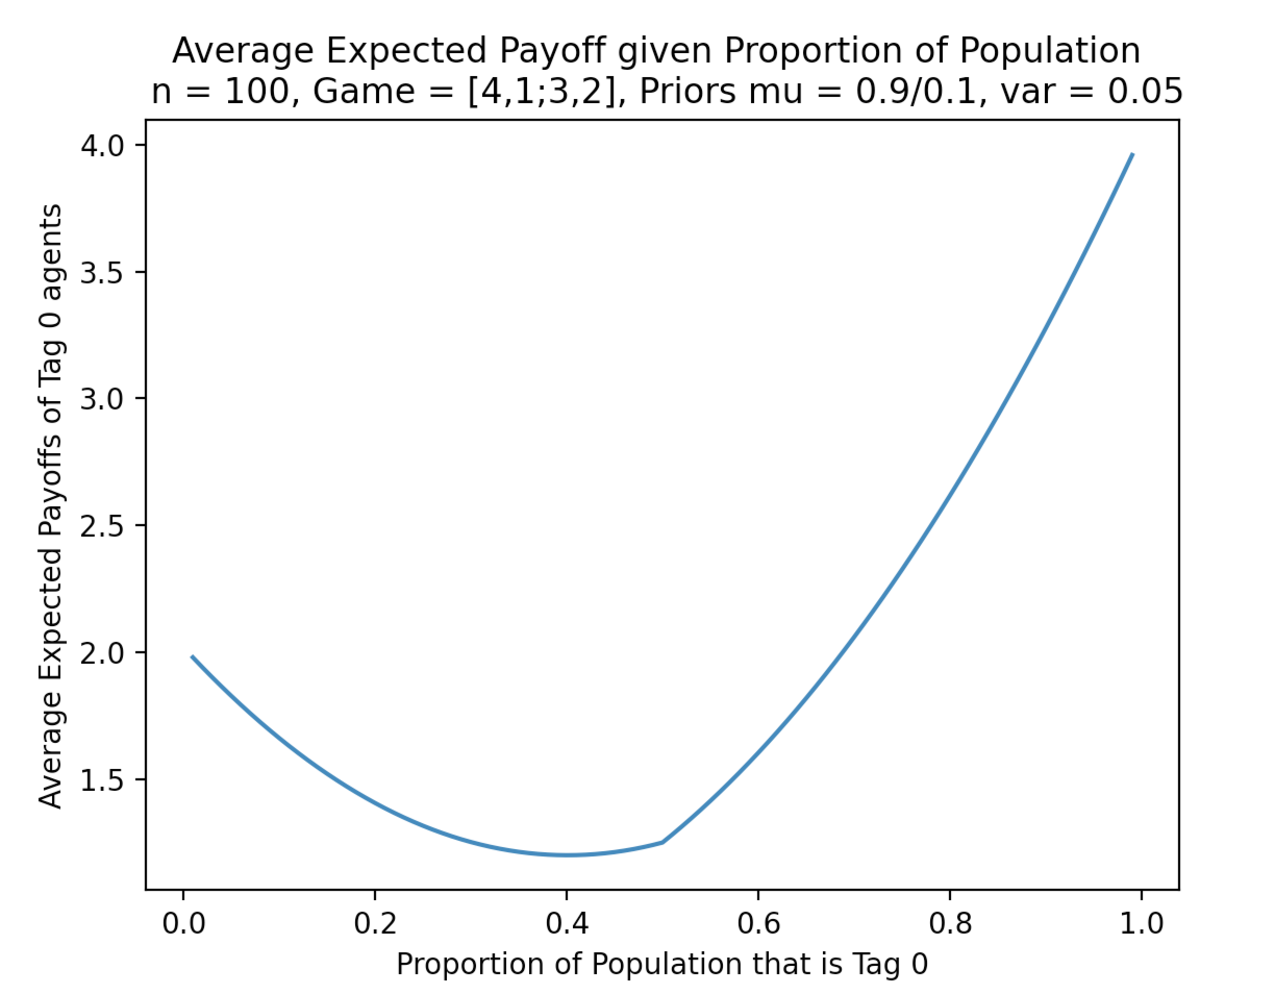
\includegraphics[width=12cm]{images/p_experiment}
%\end{figure}




\end{document}
